\documentclass[11.5pt, aspectratio=169]{beamer}
\usepackage{amsmath, amssymb, stmaryrd, mathpartir, commath, url, longtable,hyperref,tabularx}

\usepackage{forloop, microtype}
\usepackage{wasysym}
%\usepackage[dvipsnames]{xcolor}
\usepackage{csquotes}
%\usepackage{mathptmx}
\usepackage{listings}
\hypersetup{colorlinks=true,citecolor=blue}
\RequirePackage{subcaption}
\captionsetup{compatibility=false}
\usepackage{graphicx}
\usepackage{xspace}
\usepackage{dirtytalk}
\usepackage{xparse}% http://ctan.org/pkg/xparse
\usepackage{etoolbox}% http://ctan.org/pkg/etoolbox
\usepackage[framemethod=tikz]{mdframed}
\newcommand{\lambdacalc}{\ensuremath{\lambda}-calculus\xspace}
\newenvironment{fake}[1]{\par\vspace{3pt}\noindent\textbf{#1}\itshape}{\normalfont\ignorespacesafterend\vspace{3pt}\par}
\newcommand{\calcwd}[1]{\textbf{\textsf{#1}}}
\newcommand{\one}{\ensuremath{\mathbf{1}}}
\newcommand{\mvu}{\ensuremath{\lambda_{\mathsf{MVU}}}\xspace}
\newcommand{\mvupi}{\ensuremath{\lambda_{\mathsf{MVU}}^{\pi}}\xspace}
\newcommand{\app}{\:}
\newcommand{\oftype}{\: {:} \:}
\newcommand{\letin}[3]{\calcwd{let} \: #1 = #2 \: \calcwd{in} \: #3}
\newcommand{\letintwo}[2]{\calcwd{let} \: #1 = #2 \: \calcwd{in}}

\newcommand{\caseof}[2]{\calcwd{case} \: #1 \: \{ #2 \}}
\newcommand{\caseofone}[1]{\calcwd{case} \: #1 \: }
\newcommand{\midspace}{\: \mid \:}
\newcommand{\mkwd}[1]{\ensuremath{\mathsf{#1}}}
\newcommand{\antiquote}[1]{\mathbf{\{} #1 \mathbf{\}}}
\newcommand{\htmlty}[1]{\mkwd{Html}(#1)}
\newcommand{\attrty}[1]{\mkwd{Attr}(#1)}
\newcommand{\tagname}[1]{\textsf{#1}}
\newcommand{\smalllt}{\scalebox{0.85}{<}}
\newcommand{\smallgt}{\scalebox{0.85}{>}}
\newcommand{\htmltag}[3]{\smalllt \tagname{#1} \: #2 \smallgt #3 \smalllt / \tagname{#1} \smallgt}
\newcommand{\htmltagzero}[2]{\smalllt \tagname{#1} \smallgt #2 \smalllt / \tagname{#1} \smallgt}
\newcommand{\htmltagqueue}[3]{\smalllt \tagname{#1} \qsep #2 \smallgt #3 \smalllt / \tagname{#1} \smallgt}
\newcommand{\tagzero}[1]{\smalllt \tagname{#1}\smallgt}
\newcommand{\tagzeroend}[1]{\smalllt / \tagname{#1}\smallgt}
\newcommand{\opentag}[1]{\smalllt \tagname{#1}}
\newcommand{\closetag}{\smallgt}

\newcommand{\config}[1]{\mathcal{#1}}
\newcommand{\htmlterm}[1]{\calcwd{html} \app #1}
\newcommand{\attrterm}[1]{\calcwd{attribute} \app #1}
\newcommand{\seq}[1]{\overrightarrow{#1}}
\newcommand{\inl}[1]{\calcwd{inl} \: #1}
\newcommand{\inr}[1]{\calcwd{inr} \: #1}
\newcommand{\evtty}[1]{\ensuremath{\mkwd{ty}(#1)}}
\newcommand{\evt}[1]{\ensuremath{\mkwd{#1}}}
\newcommand{\qstr}[1]{\texttt{"}#1\texttt{"}}

\newcommand{\ev}{\evt{ev}\xspace}
\newcommand{\evtpayload}[2]{\evt{#1}(#2)}
\newcommand{\clickevt}{\ensuremath{\attribute{click}}}
\newcommand{\inputevt}{\ensuremath{\attribute{input}}}
\newcommand{\keydownevt}{\ensuremath{\attribute{keyDown}}}
\newcommand{\keyupevt}{\ensuremath{\attribute{keyUp}}\xspace}
\newcommand{\keypressevt}{\ensuremath{\attribute{keyPress}}\xspace}
\newcommand{\mousemoveevt}{\ensuremath{\attribute{mouseMove}}\xspace}
\newcommand{\vh}{D}
\newcommand{\pgctx}[1]{\config{D}[#1]}
\newcommand{\mh}{M\xspace}
\newcommand{\vc}{V_{\textsf{C}}\xspace}
\newcommand{\va}{V_{\textsf{a}}\xspace}

\newcommand{\ctxh}{E_{\textsf{H}}}
\newcommand{\ctxa}{E_{\textsf{a}}}

\newcommand{\state}[2]{(#1, #2)}
\newcommand{\statecomb}[3]{(#1, #2, #3)}
\newcommand{\statesub}[3]{(#1, #2, #3)}
\newcommand{\handlerproc}[3]{\langle #1 \mid #2 \mid #3 \rangle}
\newcommand{\handlerprocexp}[4]{\langle #1 \mid \state{#2}{#3} \mid #4 \rangle}
\newcommand{\handlerprocsub}[5]{\langle #1 \mid \statesub{#2}{#3}{#4} \mid #5 \rangle}
\newcommand{\idle}[1]{\calcwd{idle} \; {#1}}
\newcommand{\sys}[2]{#1 \fatsemi\: #2}
\newcommand{\sysexample}[2]{
  {\bl
  #1 \fatsemi \vspace{0.5em} \\ #2
   \el}}
\newcommand{\syssub}[4]{#1 \fatsemi\: #2 \fatsemi\: #3 \fatsemi\: #4}

\newcommand{\evalarrow}{\longrightarrow}
\newcommand{\teval}{\evalarrow_{\textsf{M}}}
\newcommand{\ceval}{\evalarrow}
\newcommand{\cevalminus}{\evalarrow_{\textsf{E}}}
\newcommand{\totheleft}[1]{\begin{flushleft}#1\end{flushleft}}
\newcommand{\evthandler}[1]{\ensuremath{\attribute{#1}}}
\newcommand{\getevthandler}[3]{#1(#2, #3)}
\newcommand{\handler}[1]{\mkwd{handler}(#1)}
\newcommand{\payload}[1]{\mkwd{payload}(#1)}
\newcommand{\id}[1]{\mkwd{id}(#1)}

\newcommand{\handle}[1]{\mkwd{handle}(#1)}

\newcommand{\defeq}{\triangleq}
\newcommand{\vdashs}{\vdash_{\textsf{T}}}
\newcommand{\ttrue}{\mkwd{true}}
\newcommand{\ffalse}{\mkwd{false}}
\newcommand{\intty}{\mkwd{Int}}
\newcommand{\boolty}{\mkwd{Bool}}
\newcommand{\stringty}{\mkwd{String}}

\newcommand{\deriv}[1]{\mathbf{#1}}
\newcommand{\produces}[1]{\:{!}\:#1}
\newcommand{\thread}[1]{(\!( #1 )\!)}
\newcommand{\wcirc}{\circ}
\newcommand{\bcirc}{\bullet}

\newcommand{\subscriptionty}[1]{\mkwd{Sub}(#1)}
\newcommand{\subscription}[2]{\calcwd{sub} \: #1 \: #2}
\newcommand{\subempty}{\calcwd{subEmpty}}
\newcommand{\emptylist}{\textbf{[}~\textbf{]}}
\newcommand{\cons}[2]{#1 :: #2}
\newcommand{\eh}{h}
\newcommand{\listty}[1]{\mkwd{List}(#1)}
\newcommand{\metadef}[1]{\mkwd{#1}}
\newcommand{\events}[1]{\metadef{events}(#1)}
\newcommand{\vs}{{V_{\mathsf{S}}}}
\newcommand{\evthandlers}[2]{\mkwd{eventHandlers}(#1, #2)}
\newcommand{\desugar}[1]{\llbracket #1 \rrbracket}

\newcommand{\gvconst}[1]{\calcwd{#1}}
\newcommand{\gvsend}[2]{\calcwd{send} \app (#1, #2)}
\newcommand{\gvrecv}[1]{\calcwd{receive} \app #1}
\newcommand{\gvcancel}[1]{\calcwd{cancel} \app #1}
\newcommand{\gvclose}[1]{\calcwd{close} \app #1}
\newcommand{\gvnew}[1]{\calcwd{new} \: #1}
\newcommand{\tryasinotherwise}[4]{\calcwd{try} \: #1 \: \calcwd{as} \: #2 \: \calcwd{in} \: #3 \: \calcwd{otherwise} \: #4}
\newcommand{\raiseexn}{\calcwd{raise}\xspace}
\newcommand{\ppos}[1]{#1^{+}}
\newcommand{\pneg}[1]{#1^{-}}
\newcommand{\gvout}[2]{{!}#1.#2}
\newcommand{\gvin}[2]{{?}#1.#2}
\newcommand{\gvoutone}[1]{{!}#1}
\newcommand{\gvinone}[1]{{?}#1}

\newcommand{\gvend}{\mkwd{End}}
\newcommand{\gvqueue}[4]{#1(#2)\leftrightsquigarrow #3(#4)}
\newcommand{\zap}[1]{\lightning #1}
\newcommand{\gvdual}[1]{\overline{#1}}
\newcommand{\without}{/}
\newcommand{\apty}[1]{\mkwd{AP}(#1)}
\newcommand{\var}[1]{\textit{#1}}


\lstdefinelanguage{Links}{%
  morekeywords={typename, fun, linfun, op, var, if, this, true, false, else, case, switch, handle,
    handler, shallowhandler, open, do, sig, new, send, receive, spawnAt, spawn,
module, request, accept, try, as, otherwise, catch, offer, select, raise,
fork, spawnClient, cancel, catch, page, close, Any, Type, Unl, forall, vdom},%
  sensitive=t, %
  comment=[l]{\#\ },%
  escapeinside={(*}{*)},%
  morestring=[d]{"},%
  keywordstyle=\color{blue},
  showstringspaces=false
  %frame = single
 }

% Links style
\lstset{
  basicstyle=\linespread{0.86}\ttfamily\small,
  keywordstyle=\bfseries,
  language=Links,
  backgroundcolor=\color{white}
}


\newcommand{\idattr}{\textit{id}\xspace}
\newcommand{\desugarterm}[1]{\llbracket #1 \rrbracket}
\newcommand{\desugarhtml}[1]{\llbracket #1 \rrbracket}
\newcommand{\desugarattr}[1]{\llbracket #1 \rrbracket}

\newcommand{\coretagone}[1]{\calcwd{htmlTag} \: \tagname{#1}}
\newcommand{\coretagtwo}[2]{\calcwd{htmlTag} \: \tagname{#1} \: #2}
\newcommand{\coretag}[3]{\calcwd{htmlTag} \: \tagname{#1} \: #2 \: #3}
\newcommand{\htmltext}[1]{\calcwd{htmlText} \: #1}
\newcommand{\htmlempty}{\calcwd{htmlEmpty}}
\newcommand{\append}[2]{#1 \star #2}

\newcommand{\attr}[2]{\calcwd{attr} \: #1 \: #2}
\newcommand{\attrempty}{\calcwd{attrEmpty}}
\newcommand{\ak}{\mathit{ak}}
\newcommand{\at}{\mathit{at}}
\newcommand{\run}[3]{\calcwd{run} \: #1 \: #2 \: #3}
\newcommand{\runsub}[4]{\calcwd{run} \: #1 \: #2 \: #3 \: #4}

\lstdefinelanguage{JavaScript}{
  morekeywords=[1]{break, continue, delete, else, for, function, if, in,
    new, return, this, typeof, var, void, while, with},
  % Literals, primitive types, and reference types.
  morekeywords=[2]{false, null, true, boolean, number, undefined,
    Array, Boolean, Date, Math, Number, String, Object, const},
  % Built-ins.
  morekeywords=[3]{eval, parseInt, parseFloat, escape, unescape},
  sensitive,
  morecomment=[s]{/*}{*/},
  morecomment=[l]//,
  morecomment=[s]{/**}{*/}, % JavaDoc style comments
  morestring=[b]',
  morestring=[b]"
}[keywords, comments, strings]

\newcommand{\bl}{\begin{array}{l}}
\newcommand{\el}{\end{array}}
\newcommand{\intstr}[1]{\mkwd{intToString}(#1)}
\newcommand{\cmdty}[1]{\mkwd{Cmd}(#1)}
\newcommand{\cmdempty}{\calcwd{cmdEmpty}}
\newcommand{\cmdspawn}[1]{\calcwd{cmdSpawn} \: #1}
\newcommand{\cmdspawnlinear}[1]{\calcwd{cmdSpawnLinear} \: #1}
\newcommand{\un}[1]{\mkwd{un}(#1)}
\newcommand{\procs}[1]{\mkwd{procs}(#1)}

\definecolor{shade}{RGB}{215,215,215}
\newcommand{\shade}[1]{\setlength{\fboxsep}{0pt}\colorbox{shade}{\vphantom{$\mid$}\ensuremath{#1}}}
%\newcommand{\shade}[1]{#1}
\newcommand{\shadetext}[1]{\setlength{\fboxsep}{0pt}\colorbox{shade}{#1}}
\newcommand{\hlred}[1]{{\color{red}{#1}}}
% \makeatletter
% \setlength{\@fptop}{0pt}
% \makeatother
\newcommand{\transition}[5]{\calcwd{transition} \: #1 \: #2 \: #3 \: #4 \: #5}
\newcommand{\transitionalone}[3]{\calcwd{transition} \: #1 \: #2 \: #3}
\newcommand{\transitionty}[2]{\mkwd{Transition}(#1, #2)}
\newcommand{\transitiontyone}[1]{\mkwd{Transition}(#1)}
\newcommand{\notransitionalone}[1]{\calcwd{noTransition} \: #1}
\newcommand{\notransition}[2]{\calcwd{noTransition} \: #1 \: #2}
\newcommand{\handlerproctrans}[4]{\handlerproc{#1}{#2}{#3}_{#4}}
\newcommand{\handlerprocexptrans}[5]{\handlerprocexp{#1}{#2}{#3}{#4}_{#5}}
\newcommand{\handlerprocexptc}[6]{\handlerprocsub{#1}{#2}{#3}{#4}{#5}_{#6}}
\newcommand{\vdashtrans}[2]{\vdash^{#1}_{#2}}
\newcommand{\threadtrans}[2]{(\!( #1 )\!)_{#2}}

\newcommand{\updating}[1]{\calcwd{updating} \: #1}
\newcommand{\extracting}[2]{\calcwd{extracting}_{#1} \: #2}
\newcommand{\extractingt}[3]{\calcwd{extractingT}_{#1, #2} \: #3}
\newcommand{\extractingtexp}[5]{\calcwd{extractingT}_{(#1, #2, #3), #4} \: #5}
\newcommand{\rendering}[2]{\calcwd{rendering}_{{#1}} \: #2}
\newcommand{\renderingext}[3]{\calcwd{rendering}_{{#1}, {#2}} \: #3}
\newcommand{\transitioning}[4]{\calcwd{transitioning}_{{#1, #2, #3}} \: #4}
\newcommand{\transitioningextexp}[6]{\calcwd{transitioning}_{{#1, #2, #3, #4, #5}} \: #6}
\newcommand{\transitioningext}[4]{\calcwd{transitioning}_{{#1, #2, #3}} \: #4}
\newcommand{\version}[1]{\mkwd{version}(#1)}

\newlength{\mylength}
\makeatletter
\newcommand{\mycfs}[1]{%
  \normalsize
  \@defaultunits\mylength=#1pt\relax\@nnil
  \edef\@tempa{{\strip@pt\mylength}}%
  \ifx\protect\@typeset@protect
     \edef\@currsize{\noexpand\mycfs\@tempa}% store calculated size
  \fi
  \mylength=1.2\mylength
  \edef\@tempa{\@tempa{\strip@pt\mylength}}%
  %\@tempa
  \expandafter\fontsize\@tempa
  \selectfont
}
\makeatother

\renewcommand{\footnotesize}{\mycfs{8}}

\newcommand{\pagety}[1]{\mkwd{Page}(#1)}
\newcommand{\pgtag}[4]{\calcwd{htmlTag}_{#4} \: \tagname{#1} \: #2 \: #3}
\newcommand{\handlers}[2]{\mkwd{handlers}(#1, #2)}
\newcommand{\diff}[2]{\mkwd{diff}(#1, #2)}

\newcommand{\redrowskip}{0.5em}
\newcommand{\qsep}{\:@\:}
\newcommand{\lin}{\mathsf{L}}
\newcommand{\unr}{\mathsf{U}}
\newcommand{\kind}{\kappa}
\newcommand{\kto}[1]{\to^{#1}}
\newcommand{\rtv}[1]{#1}
\newcommand{\recty}[2]{\mu #1 . #2}
\newcommand{\constty}[1]{\Sigma(#1)}
\newcommand{\vers}{\iota}
\newcommand{\uto}{\kto{\unr}}
\newcommand{\lto}{\multimap}
\newcommand{\halt}{\calcwd{halt}}
\newcommand{\runcomb}[5]{\calcwd{run} \: #1 \: #2 \: #3 \: #4 \: #5}
\newcommand{\ep}{E_{\textsf{P}}}
\newcommand{\tp}{T_{\textsf{P}}}
\newcommand{\domh}{D_{\mkwd{H}}}
\newcommand{\erase}[1]{\mkwd{erase}(#1)}

\newcommand{\attribute}[1]{\mkwd{#1}}
\newcommand{\textnode}[1]{\texttt{#1}}
\newcommand{\fn}[1]{\mkwd{fn}(#1)}
\usepackage{tikz-cd}

\tikzstyle{arrow} = [thick,->]
\tikzstyle{diagnode} = [rectangle, rounded corners, minimum width=4cm, minimum
height=1cm,text centered, text width=4cm, draw=black, anchor=center, fill=red!30]

\newenvironment{syntax}%
{\[\begin{array}{@{}lr@{\:\:\:}c@{\:\:\:}l}\ignorespaces}
{\end{array}\]\ignorespacesafterend}

%\definecolor{mycolor}{rgb}{0.122, 0.435, 0.698}

\newmdenv[innerlinewidth=0.5pt,linecolor=black]{mybox}

\usepackage{config/presento}
\usepackage{framed}
\usepackage{stmaryrd}
\usepackage{amsmath}
\usepackage{wasysym}
% Presento style file
\usepackage{float,lipsum}
\floatstyle{boxed}
\usepackage{mathpartir}
% custom command and packages
% custom packages
\usepackage{textpos}
\setlength{\TPHorizModule}{1cm}
\setlength{\TPVertModule}{1cm}

\newcommand\crule[1][black]{\textcolor{#1}{\rule{2cm}{2cm}}}


\usepackage{verbatim}
% Information
\title{Model-View-Update-Communicate}
\subtitle{Session Types meet the Elm Architecture}
\author{Simon Fowler}
\institute{University of Edinburgh}
\date{ABCD Final Meeting \\ 19th December 2019}

\begin{document}

% Title page
\begin{frame}[plain]
\titlepage


\hfill
\vspace{-1em}
$
\renewcommand*{\arraystretch}{1.8}
\begin{array}{r}
   
\includegraphics[height=1.5cm, keepaspectratio]{images/logos/erc-logo.jpg} \\
   
\includegraphics[height=0.7cm, keepaspectratio]{images/logos/inf_uoe.png} \\
\end{array}
$
\end{frame}

\begin{frame}{Functional Session Types}

    \begin{minipage}{0.4\textwidth}
      \[
        \mkwd{EqualityClient} \oftype \gvout{\mkwd{Int}}{\gvout{\mkwd{Int}}{\gvin{\mkwd{Bool}}{\mkwd{End}}}}
    \]
%
    \[
            \begin{array}{l}
                \mkwd{equalityClient} \oftype \mkwd{EqualityClient} \lto \mkwd{Bool} \\
                \mkwd{equalityClient}(s) \defeq \\
                \quad \letintwo{s}{\gvsend{5}{s}} \\
                \quad \letintwo{s}{\gvsend{5}{s}} \\
                \quad \letintwo{(\textit{res}, s)}{\gvrecv{s}} \\
                \quad \gvclose{s} ; \textit{res}
            \end{array}
    \]
    \end{minipage}
    \hfill
    \begin{minipage}{0.5\textwidth}
      \begin{itemize}
      \itemR Session types: Types for protocols
      \itemR Here, interested in \emph{linear functional languages}
      \itemR Huge advances over the course of ABCD!
    \end{itemize}
    \end{minipage}
\end{frame}

\begin{frame}{Interactivity?}

  \begin{fullpageitemize}
  \item {\Large \textbf{Majority of implementations: Command line applications}}
  \end{fullpageitemize}
  \vspace{-1em}
  \begin{center}
    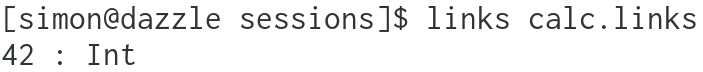
\includegraphics[width=0.75\textwidth]{images/batch-prog.png}
  \end{center}
  \vspace{1.5em}

  \begin{fullpageitemize}
    \item Really, communication actions triggered by UI events, sending user-specified data
    \item \emph{Difficult to embed linear resources into a GUI}
    \item Some early work on session types + GUIs, but ad-hoc, not formal
      \begin{itemize}
        \itemR (Client code in Exceptional Asynchronous Session Types was a \emph{mess})
      \end{itemize}
  \end{fullpageitemize}
\end{frame}

\begin{frame}[plain]
  \begin{center}
    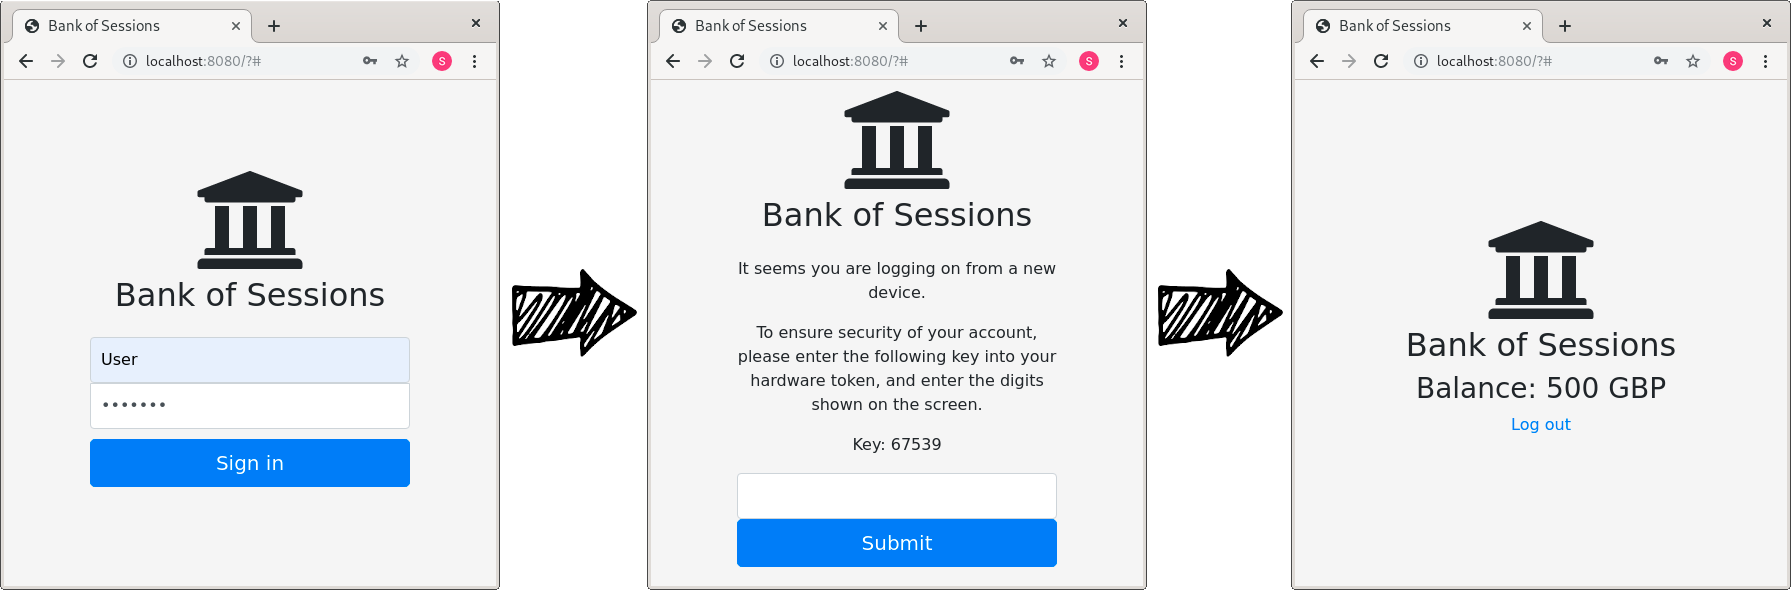
\includegraphics[width=0.7\textwidth]{images/2fa.png}
  \end{center}
  \pause

\[
    \def\arraystretch{1.25}
\bl
  \metadef{TwoFactorClient} \defeq \\
  \quad\gvoutone{(\mkwd{Username}, \mkwd{Password})} . \textit{\&} \{ \\
  \qquad \mkwd{Authenticated}: \metadef{ClientBody}, \\
  \qquad \mkwd{Challenge}: \gvinone{\mkwd{ChallengeKey}} .
    \gvoutone{\mkwd{Response}} . \textit{\&} \{
    \begin{aligned}[t]
      & \mkwd{Authenticated}: \metadef{ClientBody}, \\
    & \mkwd{AccessDenied}: \gvend \},
    \end{aligned} \\
  \qquad \mkwd{AccessDenied}: \gvend \\
  \quad \}
\el
\]

\end{frame}


\begin{frame}{Approach}

  \begin{minipage}{0.25\textwidth}
      
\includegraphics[width=\textwidth]{images/ElmLogo.png}
  \end{minipage}
  \hfill
  \begin{minipage}{0.7\textwidth}
    {\large \textbf{Step 1: Formalise a GUI framework}}
    \begin{itemize}
      \itemR I chose Model-View-Update, as pioneered by Elm
    \end{itemize}
  \end{minipage}

  \vspace{2em}

  \begin{minipage}{0.25\textwidth}
    \begin{center}
      \scalebox{2.5}{\Huge $\pi$}
    \end{center}
  \end{minipage}
  \hfill
  \begin{minipage}{0.7\textwidth}
    {\large \textbf{Step 2: Extend formalism with session types}}
   \begin{itemize}
   \itemR Some intricacies...
   \end{itemize}
  \end{minipage}

  \vspace{2em}

  \begin{minipage}{0.25\textwidth}
    \begin{center}
      
\includegraphics[width=0.5\textwidth]{images/links-logo.png}
    \end{center}
  \end{minipage}
  \hfill
  \begin{minipage}{0.7\textwidth}
    {\large \textbf{Step 3: Implement in Links}}
    \begin{itemize}
    \itemR Result: Idiomatic server \emph{and} client code for session-typed web applications
    \end{itemize}
  \end{minipage}
\end{frame}

\begin{frame}{Contributions}
  \begin{fullpageitemize}
  \item {\Large \textbf{\mvu: A Formal Model of the MVU Architecture}}
    \begin{itemize}
      \itemR First formal characterisation of MVU
      \itemR Soundness proofs
    \end{itemize}
    \vspace{0.25em}

  \item {\Large \textbf{Extending \mvu with Session Types}}
    \begin{itemize}
      \itemR Formal characterisations of \emph{subscriptions} and \emph{commands} from Elm
      \itemR \emph{Linearity} and \emph{model transitions} allow safe integration of session types
    \end{itemize}
    \vspace{0.25em}

  \item {\Large \textbf{Implementation and Examples}}
    \begin{itemize}
      \itemR MVU + extensions implemented in Links language
      \itemR Example applications including two-factor authentication and chat server
    \end{itemize}
  \end{fullpageitemize}
\end{frame}

\framecard{{\color{white}\bigtext{Demo: A box and a label}}}

\begin{frame}{Model-View-Update}

  \begin{center}
    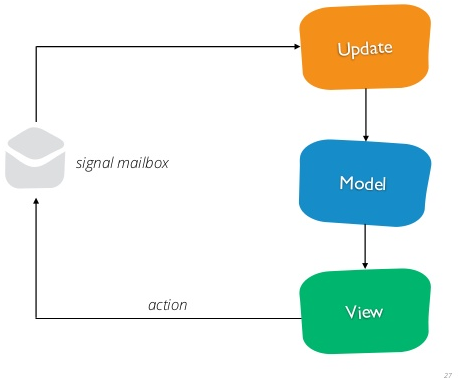
\includegraphics[scale=1.3]{images/mvu.png}

    \hfill {\tiny \url{https://www.slideshare.net/RogerioChaves1/introduction-to-elm}}
  \end{center}

  \begin{fullpageitemize}
  \item {\Large \textbf{Model}: State of application}
  \item {\Large \textbf{View}: Renders model as HTML}
  \item {\Large \textbf{Update}: Updates model based on UI messages}
  \end{fullpageitemize}

\end{frame}

\begin{frame}[fragile]{Model-View-Update (in Links)}

\setbeamercovered{transparent}
\vspace{-1em}
\begin{overlayarea}{\linewidth}{10cm}
\begin{uncoverenv}<1->
\begin{lstlisting}[language=Links]
typename Model   = (contents: String);
typename Message = [| UpdateBox: String |];
\end{lstlisting}
\end{uncoverenv}

\begin{uncoverenv}<2->
\begin{lstlisting}[language=Links]
sig view : (Model) ~> HTML(Message)
fun view(model) {
 vdom
  <input
    type="text" value="{model.contents}"
    e:onInput="{fun(str) { UpdateBox(str) }}"/>
  <div>{ textNode(reverse(model.contents)) }</div>
}
\end{lstlisting}
\end{uncoverenv}

  \begin{uncoverenv}<3->
\begin{lstlisting}[language=Links]
sig updt : (Message, Model) ~> Model
fun updt(UpdateBox(newStr), model) {
  (contents = newStr)
}
\end{lstlisting}
\end{uncoverenv}

  \begin{uncoverenv}<4->
\begin{lstlisting}[language=Links]
mvuPage((contents=""), view, updt)
\end{lstlisting}
\end{uncoverenv}
\end{overlayarea}
\end{frame}

\framecard{{\color{white}\bigtext{$\mvu$: Model-View-Update, Formally}}}

\begin{frame}{Syntax}

  {\large
  \begin{syntax}
  \text{Types} & A, B, C & ::= & \one \midspace A \to B \midspace A \times B
  \midspace A + B \midspace \stringty \midspace \intty \\
               &      & \midspace & \shade{\htmlty{A}} \midspace \shade{\attrty{A}} \\
%\text{Base types} & C & ::= & \mkwd{String} \midspace \mkwd{Int} \\
\text{String literals} & s \\
\text{Integers} & n \\
%\text{Booleans} & b & ::= & \ttrue \midspace \ffalse \\
\text{Terms} & L, M, N & ::= &
  % Basic lambda calculus
  x \midspace \lambda x . M \midspace M \app N \midspace () \midspace s \midspace n \\
  & & \midspace & (M, N) \midspace \letin{(x, y)}{M}{N} \\
  & & \midspace & \inl{x} \midspace \inr{x} \midspace \caseof{L}{\inl{x} \mapsto M; \inr{y} \mapsto N} \\
  & & \midspace & \shade{\coretag{t}{M}{N}} \midspace \shade{\htmltext{M}} \midspace \shade{\htmlempty} \\
  & & \midspace & \shade{\attr{\ak}{M}} \midspace \shade{\attrempty} \midspace \shade{\append{M}{N}} \\
  \end{syntax}

    \[
  \begin{array}{llp{3em}lrcl}
    \shade{\text{Tag names}} & \shade{\tagname{t}} & & \shade{\text{Attribute keys}} & \shade{\ak} & ::= & \shade{\mathit{at}} \midspace \shade{\mathit{h}} \\
    \shade{\text{Attribute names}} \:\: & \shade{\mathit{at}} & & \shade{\text{Event handler names}} & \shade{\mathit{h}}
     % & & \text{Attributes} & a & ::= & \textit{ak} = \textit{ab}\\
    % \text{HTML} & H & ::= & \htmltag{t}{\seq{a}}{\seq{H}} \midspace s \midspace \antiquote{M} \\
    \end{array}
  \]%
}
\end{frame}

\begin{frame}{Syntactic Sugar}

    \[
      \left\llbracket
    \begin{array}{l}
      \calcwd{html} \\
      %\mkwd{view} \defeq \lambda \textit{model} . \calcwd{html} \\
      \quad \opentag{input} \: \attribute{type}=\textnode{"text"} \:
      \attribute{value} = \{ \var{model}.\var{contents} \} \\
      \qquad
        \attribute{onInput} = \{ \lambda \textit{str}.
          \mkwd{UpdateBox}(\textit{str})\} \closetag \tagzeroend{input}  \\
          %
        \quad \htmltagzero{div}{\antiquote{\htmltext{(\metadef{reverseString} \:
        (\textit{model}. \textit{contents}))}}}
    \end{array}
    \right\rrbracket
  \]%
  \vspace{0.25em}
  {\Huge
  \[
    =
  \]%
}
  %\vspace{1em}
  \[
    \begin{array}{l}
        (\coretagone{input} \\
        \quad ((\attr{\attribute{type}}{\textnode{"text"}}) \star
        (\attr{\attribute{value}}{\var{model}.\var{contents}}) \star \\
         \qquad
         (\attr{\attribute{onInput}}{(\lambda \textit{str}.
         \mkwd{UpdateBox}(\textit{str})}))) \: \htmlempty) \: \star \\
         \quad
         \coretag{div}{\attrempty}{(\htmltext{\metadef{reverseString} \:
         (\textit{model}.\textit{contents}}))}
    \end{array}
  \]
\end{frame}

% \begin{frame}{Runtime Syntax}
%
% \end{frame}

\begin{frame}{Semantics by example: Box and a label}

  \large
\[
      \bl
      \mkwd{model} \defeq (\var{contents} = \textnode{""}) \vspace{2em} \\
      \mkwd{view} \defeq \lambda \textit{model} . \calcwd{html} \\
      \quad \opentag{input} \: \attribute{type}=\textnode{"text"} \:
      \attribute{value} = \{ \var{model}.\var{contents} \} \\
      \qquad
        \attribute{onInput} = \{ \lambda \textit{str}.
          \mkwd{UpdateBox}(\textit{str})\} \closetag \tagzeroend{input}  \\
          %
        \quad \htmltagzero{div}{\antiquote{\htmltext{(\metadef{reverseString} \:
        (\textit{model}. \textit{contents}))}}} \vspace{2em} \\
        %
        \mkwd{update} \defeq \lambda \mkwd{UpdateBox}(\var{str}) . (\var{contents} = \var{str})
      \el
    \]
\end{frame}

\begin{frame}{Semantics by example: Box and a label}

  \large
\begin{overlayarea}{\linewidth}{5cm}
  \[
  \only<1>{
     \run{\mkwd{model}}{\mkwd{view}}{\mkwd{update}}
  }
  %
  \only<2>{
    \sysexample{\handlerprocexp{(\mkwd{model}, \mkwd{view} \app \mkwd{model})}{\mkwd{view}}{\mkwd{update}}{\epsilon}}{\htmlempty}
  }
  %
  \only<3>{
    \sysexample{\handlerprocexp{(\mkwd{model},
        \bl
        \opentag{input} \: \attribute{type}=\textnode{"text"} \:
          \attribute{value}=\textnode{""} \\
            \quad  \attribute{onInput} = \{ \lambda \var{str}.
              \mkwd{UpdateBox}(\var{str})\} \closetag \\
              \tagzeroend{input}  \\
               \htmltagzero{div}{}
        \el
      )}{\mkwd{view}}{\mkwd{update}}{\epsilon}}{\htmlempty}
  }
  %
  \only<4>{
      \sysexample{\handlerprocexp{\idle{\mkwd{model}}}{\mkwd{view}}{\mkwd{update}}{\epsilon}}{
      {\bl
        \opentag{input} \: \attribute{type}=\textnode{"text"} \:
        \attribute{value}=\textnode{""} \\
          \quad  \attribute{onInput} = \{ \lambda \var{str}.
            \mkwd{UpdateBox}(\var{str})\} \qsep \epsilon \closetag \tagzeroend{input}  \\
            \htmltagqueue{div}{\epsilon}{}
      \el}
    }
  }
  %
  \only<5>{
        \sysexample{\handlerprocexp{\idle{\mkwd{model}}}{\mkwd{view}}{\mkwd{update}}{\epsilon}}{
      \bl
      \opentag{input} \: \attribute{type}=\textnode{"text"} \:
      \attribute{value}=\textnode{""} \\
              \quad \attribute{onInput} = \{ \lambda \var{str}.
              \mkwd{UpdateBox}(\var{str})\} \qsep \evtpayload{click}{()} \cdot \\
              \quad \evtpayload{keyDown}{75} \cdot \evtpayload{keyUp}{75} \cdot
              \evtpayload{input}{\textnode{"k"}}\closetag \tagzeroend{input} \\
              \htmltagqueue{div}{\epsilon}{}
      \el
    }
  }
  %
  \only<6>{
    \sysexample{\handlerprocexp{\idle{\mkwd{model}}}{\mkwd{view}}{\mkwd{update}}{\epsilon}}{
        \bl
        \opentag{input} \: \attribute{type}=\textnode{"text"} \:
        \attribute{value}=\textnode{""} \\
                \quad \attribute{onInput} = \{ \lambda \var{str}.
                \mkwd{UpdateBox}(\var{str})\} \qsep
                  \evtpayload{input}{\textnode{"k"}}\closetag
                  \\ \tagzeroend{input} \\
                \htmltagqueue{div}{\epsilon}{}
        \el
    }
  }
  %
  \only<7>{
\sysexample{\handlerprocexp{\idle{\mkwd{model}}}{\mkwd{view}}{\mkwd{update}}{\epsilon} \parallel
          \thread{\mkwd{UpdateBox}(\textnode{"k"})}}{
        \bl
        \opentag{input} \: \attribute{type}=\textnode{"text"} \:
        \attribute{value}=\textnode{""} \\
                \quad \attribute{onInput} = \{ \lambda \var{str}.
                \mkwd{UpdateBox}(\var{str})\}
                \\ \qsep \epsilon \closetag \tagzeroend{input} \\
                \htmltagqueue{div}{\epsilon}{}
        \el
    }
  }
  %
  \only<8>{
\sysexample{\handlerprocexp{\idle{\mkwd{model}}}{\mkwd{view}}{\mkwd{update}}{\mkwd{UpdateBox}(\textnode{"k"})}}{
        \bl
        \opentag{input} \: \attribute{type}=\textnode{"text"} \:
        \attribute{value}=\textnode{""} \\
                \quad \attribute{onInput} = \{ \lambda \var{str}.
                \mkwd{UpdateBox}(\var{str})\}
                \\ \qsep \epsilon \closetag \tagzeroend{input} \\
                \htmltagqueue{div}{\epsilon}{}
        \el
      }
  }
  %
  \only<9>{
      \sysexample{\handlerprocexp{\handle{\mkwd{model}, (\mkwd{view}, \mkwd{update}), \mkwd{UpdateBox}(\textnode{"k"})}}{\mkwd{view}}{\mkwd{update}}{\epsilon}}{
        \bl
        \opentag{input} \: \attribute{type}=\textnode{"text"} \:
        \attribute{value}=\textnode{""} \\
                \quad \attribute{onInput} = \{ \lambda \var{str}.
                \mkwd{UpdateBox}(\var{str})\}
                \\ \qsep \epsilon \closetag \tagzeroend{input} \\
                \htmltagqueue{div}{\epsilon}{}
        \el
      }
      % This hack almost feels like an SQL injection attack
    \]

    \vspace{1em}
      \[
        (\text{where }
        \handle{m, (v, u), \var{msg}} \defeq \letin{m'}{u \app (\var{msg}, m)}{(m', v \app m')})
  }
  %
  \only<10>{
          \sysexample{\handlerprocexp{(
    \bl
      (\var{contents}=\textit{"k"}), \\
       \quad \opentag{input} \: \attribute{type}=\textnode{"text"} \:
         \attribute{value}=\textnode{"k"} \\
        \qquad  \attribute{onInput} = \{ \lambda \var{str}.
           \mkwd{UpdateBox}(\var{str})\} \closetag \\
        \quad \tagzeroend{input}  \\
           \quad  \htmltagzero{div}{k} \\
    \el
        )}{\mkwd{view}}{\mkwd{update}}{\epsilon}}{
        \bl
        \opentag{input} \: \attribute{type}=\textnode{"text"} \:
        \attribute{value}=\textnode{""} \\
                \quad \attribute{onInput} = \{ \lambda \var{str}.
                \mkwd{UpdateBox}(\var{str})\}
                \\ \qsep \epsilon \closetag \tagzeroend{input} \\
                \htmltagqueue{div}{\epsilon}{}
        \el
      }
  }
  %
    \only<11>{
      \sysexample{\handlerprocexp{\idle{\;(\textit{contents}=\textnode{"k"})}}{\mkwd{view}}{\mkwd{update}}{\epsilon}}
      { {\bl
     \opentag{input} \: \attribute{type}=\textnode{"text"} \:
     \attribute{value}=\textnode{"k"} \\
       \quad  \attribute{onInput} = \{ \lambda \var{str}.
         \mkwd{UpdateBox}(\var{str})\} \qsep \epsilon \closetag \tagzeroend{input}  \\
         \htmltagqueue{div}{\epsilon}{\textnode{k}}
  \el}
  }
    }
\]
\end{overlayarea}
\end{frame}

\begin{frame}{Metatheory}


\begin{theorem}[Preservation]\label{thm:config-pres}
  If $\Gamma \vdash \config{C}$ and $\config{C} \ceval \config{C}'$, then $\Gamma \vdash \config{C}'$.
\end{theorem}

\vspace{1em}

\begin{theorem}[Event Progress]\label{thm:event-progress}
  If $\cdot \vdash \config{C}$, either:
  \begin{itemize}
    \itemR there exists some $\config{C}'$ such that $\config{C} \cevalminus
      \config{C'}$; or
    \itemR $\config{C} = \sys{\handlerprocexp{\idle{V_m}}{V_v}{V_u}{\epsilon}}{\vh}$ where $\vh$
      cannot be written $\config{D}[\pgtag{t}{V}{W}{\seq{e}}]$ for some
      non-empty $\seq{e}$.
    \end{itemize}
\end{theorem}

\end{frame}

\framecard{{\color{white}\bigtext{Extending $\mvu$}}}

\begin{frame}{Commands}

  \begin{fullpageitemize}
  \item \textbf{Commands}: Allow side effects to be performed by event loop
  \item Example: Asynchronous na\"ive Fibonacci
  \end{fullpageitemize}

  {\small
    \onslide<2->{
  \[
\bl
\mkwd{Model} \defeq \mkwd{Maybe}(\intty) \qquad
\mkwd{Message} \defeq \mkwd{StartComputation} \midspace \mkwd{Result}(\intty) \vspace{0.75em}
\el
\]
}
%
%\mkwd{model} : \mkwd{Model} \\
%\mkwd{model} \defeqw (0, 0) \\ \\
%
\onslide<3->{
\[
  \bl
\mkwd{view} : \mkwd{Model} \to \htmlty{\mkwd{Message}} \\
\mkwd{view} = \lambda \var{model} . \calcwd{html} \\
\quad \{
  \caseofone{model} \{ \\
  \qquad
  {\begin{array}[t]{l}
     \mkwd{Just}(\textit{result}) \mapsto \htmltext{\intstr{x}}; \\
     \mkwd{Nothing} \mapsto \htmltext{\textnode{"Waiting \ldots"}} \:
   \}
  \quad \} \\
  \end{array}} \\
  \quad \htmltag{button}{\attribute{onClick} = \antiquote{\lambda () .
  \mkwd{StartComputation}} }{\textnode{Start!}} \vspace{0.75em} \\
\el
\]%
}
\onslide<4->{
\[
  \bl
\mkwd{update} : (\mkwd{Message} \times \mkwd{Model}) \to (\mkwd{Model},
\cmdty{\mkwd{Message}})\\
\mkwd{update} = \lambda \textit{model} . \\
\quad \caseofone{\textit{model}} \{ \\
  \qquad \mkwd{StartComputation} \mapsto (\mkwd{Nothing},
  \cmdspawn{\mkwd{Result}(\textsf{na\"iveFib}(1000))}) \\
  \qquad \mkwd{Result}(x) \mapsto (\mkwd{Just}(x), \cmdempty) \\
  \quad \}
\el
\]%
}
}
\end{frame}

\begin{frame}{Linearity}

  \begin{fullpageitemize}
  \item Stock \mvu does not support linearity (as $m'$ is used non-linearly when calculating new model and view):
  \end{fullpageitemize}
  \[
    \handle{m, (v, u), \var{msg}} \defeq \letin{m'}{u \app m}{(\hlred{m'}, v \app \hlred{m'})}
  \]%
  \vspace{0.25em}
  \begin{fullpageitemize}
  \itemR Idea: linear parts of model only used in update, not view. \\
    \emph{Extract} unrestricted part of the model:
  \end{fullpageitemize}
  \begin{mybox}
  \[
    \begin{array}{lcl}
      \mkwd{extract} & : & \mkwd{Model} \to (\mkwd{Model} \times \mkwd{UnrestrictedModel}) \\
      \mkwd{view}    & : & \mkwd{UnrestrictedModel} \to \htmlty{\mkwd{Message}} \\
    \end{array}
  \]
\[
\begin{array}{l}
  \handle{\textit{m}, (\textit{v}, \textit{u}, \textit{e}), \textit{msg}}
  \defeq
    \begin{aligned}[t]
      & \letintwo{m'}{u \app (\textit{msg}, m)} \\
      & \shade{\letintwo{(m', \textit{unrM})}{e \app m'}} \\
      & {(m', v \app \shade{\textit{unrM}})}
    \end{aligned}
  \end{array}
\]
\end{mybox}

% \begin{center}
%   (Remainder of machinery for integrating linear / unrestricted types standard)
% \end{center}
\end{frame}

\framecard{{\color{white}\bigtext{Demo: PingPong application}}}

\begin{frame}{PingPong in $\mvu$}

\setbeamercovered{transparent}
  {\small
    \begin{minipage}[t]{0.45\textwidth}
      \[
        \bl
        \mkwd{PingPong} \defeq \mu t . {!}\mkwd{Ping} . {?}\mkwd{Pong} . t \vspace{0.5em} \\
        \mkwd{Model} \defeq \mkwd{Pinging}(\mkwd{PingPong}) \midspace \mkwd{Waiting} \\
        \mkwd{Message} \defeq \mkwd{Click} \midspace \mkwd{Ponged}(\mkwd{PingPong})
        \el
      \]%
    \end{minipage}
    \hfill
    \begin{minipage}[t]{0.475\textwidth}
\[
   \bl
  \mkwd{update} \defeq  \lambda (\textit{msg}, \textit{model}) . \\
  \quad \caseofone{\textit{msg}} \{ \\
    \qquad \mkwd{Click} \mapsto \mkwd{handleClick}(\var{model}) \\
    \qquad \mkwd{Ponged}(c) \mapsto \mkwd{handlePonged}(\var{model}, c) \\
      \quad \}
  \el
\]
    \end{minipage}
    \onslide<2>{
\begin{minipage}[t]{0.6\textwidth}
\[
  \bl
  \mkwd{handleClick}(\var{model}) \defeq \\
  \quad \caseofone{\var{model}} \{ \\
    \qquad \mkwd{Pinging}(c) \mapsto \\
    \quad \qquad \letintwo{c}{\gvsend{\mkwd{Ping}}{c}} \\
    \quad \qquad \calcwd{let} \: {\var{cmd}} = \\
    \quad \qquad \quad {\cmdspawn{(
         {\begin{aligned}[t]
         & \letintwo{(\var{pong}, c)}{\gvrecv{c}} \\
         & {\mkwd{Ponged}(c)}) \: \calcwd{in}
    \end{aligned}}}}  \\
    \qquad \quad (\mkwd{Waiting}, \var{cmd}) \\
    \qquad \hlred{\mkwd{Waiting} \mapsto (\mkwd{Waiting}, \cmdempty)} \\
   \quad \}
   \el
\]
\end{minipage}
\hfill
\begin{minipage}[t]{0.35\textwidth}
\[
  \bl
  \mkwd{handlePonged}(\var{model}, c) \defeq \\
    \quad \caseofone{\var{model}} \{ \\
      \qquad \hlred{\mkwd{Pinging}(c') \mapsto} \\
      \qquad \quad \hlred{\gvcancel{c'};} \\
      \qquad \quad \hlred{(\mkwd{Pinging}(c), \cmdempty)} \\
       \qquad \mkwd{Waiting} \mapsto \\
       \qquad \quad (\mkwd{Pinging}(c), \cmdempty) \\
     \quad \}
   \el
 \]
\end{minipage}
}
}
\end{frame}

\begin{frame}{Illegal states}
  \begin{fullpageitemize}
    \item {\LARGE \textbf{Issue}}
      \begin{itemize}
        \itemR Must handle messages impossible in a given state
          (e.g., receiving a pong while waiting to send a ping)
        \itemR Problem: models treated as sum types
      \end{itemize}
      \vspace{0.25em}
    \item {\LARGE \textbf{Proposal}}
      \begin{itemize}
        \itemR \emph{Multiple} model types, \emph{transitions} between them
        \itemR Make illegal states unrepresentable!
      \end{itemize}
  \end{fullpageitemize}
\end{frame}

\begin{frame}{Model transitions}
\setbeamercovered{transparent}
  \small
    \framebox{
\begin{minipage}[t]{0.4\textwidth}
  \begin{center}
    \mkwd{Waiting} \text{state}
  \end{center}
  \vspace{-1em}
  \[
  \bl
  \mkwd{WModel} \defeq \mkwd{Waiting} \\
  \mkwd{WUModel} \defeq \one \\
  \mkwd{WMessage} \defeq \mkwd{Ponged}(c) \\ \\
  %
  \mkwd{wView} \defeq \lambda \var{()} . \: \calcwd{html} \\
  \quad \opentag{button} \: \attribute{disabled}=\textnode{"true"} \closetag \\
  \qquad \textnode{Send Ping!} \\
  \quad \tagzeroend{button} \\ \\
  %
  \mkwd{wUpdate} \defeq \lambda(\mkwd{Ponged}(c), \mkwd{Waiting}) . \\
  \quad
  \calcwd{transition} \: {\mkwd{Pinging}(c)} \: {\mkwd{pView}} \\
  \qquad {\mkwd{pUpdate}} \: {\mkwd{pExtract}} \: {\cmdempty} \\ \\
  %
  \mkwd{wExtract} \defeq \lambda x . (\mkwd{Waiting}, ())
  \\
  \vspace{0.3em}
  \el
  %
  \]
\end{minipage}
}
\hfill
\onslide<2>{
\framebox{
\begin{minipage}[t]{0.5\textwidth}
  \begin{center}
  \mkwd{Pinging} \text{state}
  \end{center}
  \vspace{-1em}
  \[
  \bl
  \mkwd{PModel} \defeq \mkwd{Pinging}(\mkwd{PingPong}) \\
  \mkwd{PUModel} \defeq \one \\
  \mkwd{PMessage} \defeq \mkwd{Click}
  \vspace{0.275em} \\
  %
  \mkwd{pView} \defeq \lambda () . \: \calcwd{html} \\
    \quad \opentag{button} \: {\attribute{onClick} = \antiquote{\lambda () . \mkwd{Click}}} \closetag \\
    \qquad \textnode{Send Ping!} \\
    \quad \tagzeroend{button} \vspace{0.4em} \\
    %
\mkwd{pUpdate} \defeq \lambda (\mkwd{Click}, \mkwd{Pinging}(c)) . \\
\quad \letintwo{c}{\gvsend{\mkwd{Ping}}{c}} \\
    \quad \calcwd{let} \: {\var{cmd}} = \\
    \qquad {\cmdspawn{(
         {\begin{aligned}[t]
         & \letintwo{(\var{pong}, c)}{\gvrecv{c}} \\
         & {\mkwd{Ponged}(c)}) \: \calcwd{in}
    \end{aligned}}}}  \\
    \quad
    \transition{()}{\mkwd{wView}}{\mkwd{wUpdate}}{\mkwd{wExtract}}{\var{cmd}}
    \vspace{0.4em} \\
    \mkwd{pExtract} \defeq \lambda c . (c, ())
  \el
  \]
\end{minipage}
}
}
\end{frame}

\framecard{{\color{white}\bigtext{Wrapping up}}}

\begin{frame}{Conclusion}

  \begin{fullpageitemize}

  \item {\LARGE{\textbf{Summary}}}
    \begin{itemize}
      \itemR First formal characterisation of MVU architecture
      \itemR First formal integration of session-typed communication and GUI programming
      \itemR Not only Greek: fully implemented in Links, along with examples
    \end{itemize}
    \vspace{1em}
  \item {\LARGE{\textbf{Find out more!}}}
      \begin{itemize}
        \itemR Draft paper: \url{http://bit.ly/mvu-arxiv}
        \itemR Artifact: \url{http://bit.ly/mvu-artifact}
      \end{itemize}
  \end{fullpageitemize}
 \vspace{1em}
  \centering
  \texttt{@Simon\_JF}

  \centering
  \texttt{simon.fowler@ed.ac.uk}

  \centering
  \url{http://www.links-lang.org}

  \centering
  \texttt{opam install links}

\end{frame}

\end{document}

